% !TEX encoding = UTF-8
% !TEX TS-program = pdflatex
% !TEX root = ../../tesi.tex

\subsection{Vincoli tecnologici}
In questa sezione vengono presentati gli strumenti e le tecnologie decise ed utilizzate per procedere al meglio durante la fase di sviluppo.

\subsubsection{Strumenti di gestione del progetto}
Il processo di sviluppo è molto complicato e articolato, in quanto riguarda molte fasi che fanno comunicare numerose persone. Per questo è importante scegliere gli strumenti adeguati che riescano ad accompagnare questo processo, semplificandolo ed automatizzando alcune parti di esso. Di seguito verranno spiegati quali strumenti per la gestione del progetto ho scelto e soprattutto il perché.

\paragraph{Version Control System}
I VCS (\textit{Version Control System}) sono strumenti che registrano tutte le modifiche che avvengono in un insieme di \textit{file}, favorendone la condivisione. Quello che è stato scelto per questo progetto è \textbf{Git}, uno strumento per il controllo del versionamento del \textit{software} in maniera distribuita, o anche comunemente chiamato \textit{DVCS} (\textit{Distributed Version Control System}). Git può essere utilizzato da riga di comando, come ho fatto io, oppure attraverso vari \textit{client} grafici che ne facilitano l'uso. \\

In Git ogni modifica rappresenta un \textit{commit}, al quale viene associato un codice univoco dato dallo stato attuale dei \textit{file} e dall'orario di effettuazione. Una \textit{repository} Git permette di dividere il codice in vari ambienti di lavoro anche detti \textit{branch}. Un \textit{branch} non è altro che un semplice puntatore ad un \textit{commit}, dal quale può iniziare una storia diversa del codice. Questi \textit{branch} possono essere fusi, attraverso il processo di \textit{merging}, e chiusi. È possibile anche creare dei \textit{tag} associati ad un \textit{commit}, ovvero dei puntatori immutabili che spesso vengono utilizzati per rilasciare la nuova versione di un \textit{software}. \\

Tra le tante caratteristiche di Git è presente il fatto di essere distribuito. Infatti, quando viene importata una \textit{repository} Git all'interno di un ambiente locale, come può essere un \textit{computer}, questa si porterà dietro tutta la storia delle modifiche del \textit{software} dal primo commit in poi. Questo porta molti vantaggi, tra cui una migliore risoluzione dei conflitti, possibilità di continuare il proprio lavoro anche se il nodo centrale non risponde, visto che non è presente un nodo principale, e anche la possibilità di impostare diversi \textit{workflow} che non sono possibili nei VCS centralizzati. 

\paragraph{Git workflow}
Un Git \textit{workflow} è un insieme di regole che dicono come svolgere il lavoro in modo coerente e produttivo,  aiutando lo sviluppo del \textit{software} e facilitando l'utilizzo di pratiche di \textit{DevOps} e di \textit{Continuous Integration}. Il \textit{workflow} che è stato utilizzato è \textbf{un misto tra GitFlow e GitHub Flow}.
L'idea alla base di questo \textit{workflow} è il fatto di avere due \textit{branch} che mantengono la storia del progetto: il \textit{main} e il \textit{develop}. Il \textit{branch main} ha il compito di storicizzare tutti i rilasci ufficiali, mentre il \textit{branch develop} è un branch di integrazione per le nuove funzionalità che dovranno essere aggiunte alla nuova versione del \textit{software}. Ogni nuova funzionalità da aggiungere al \textit{software} deve essere sviluppata in un opportuno \textit{feature branch}, che in seguito verrà integrato con il \textit{develop} dopo l'approvazione della \textit{pull request}.

Una volta che il \textit{branch develop} ha acquisito abbastanza nuove funzionalità per un rilascio, da quest'ultimo verrà creato un nuovo \textit{branch} di tipo \textit{release}, dove si potrà perfezionare il codice eseguendo gli ultimi \textit{test} o \textit{bugfix}, per poi essere fuso dentro il \textit{branch main} e il \textit{branch develop}. In seguito verrà anche associato un \textit{tag} all'ultimo \textit{commit} del \textit{branch main}, in modo tale da consolidare la nuova versione del \textit{software}.
Un'altra categoria importante di \textit{branch} sono quelli chiamati \textit{HotFix}, che servono per eseguire dei \textit{fix} al codice che è già stato integrato in una \textit{release}. Questo tipo di \textit{branch} ha il compito di riparare l'errore sia nel \textit{branch main} e sia nel \textit{branch develop}, attraverso la fusione in entrambi.

\begin{figure}[h!]
  \centering
  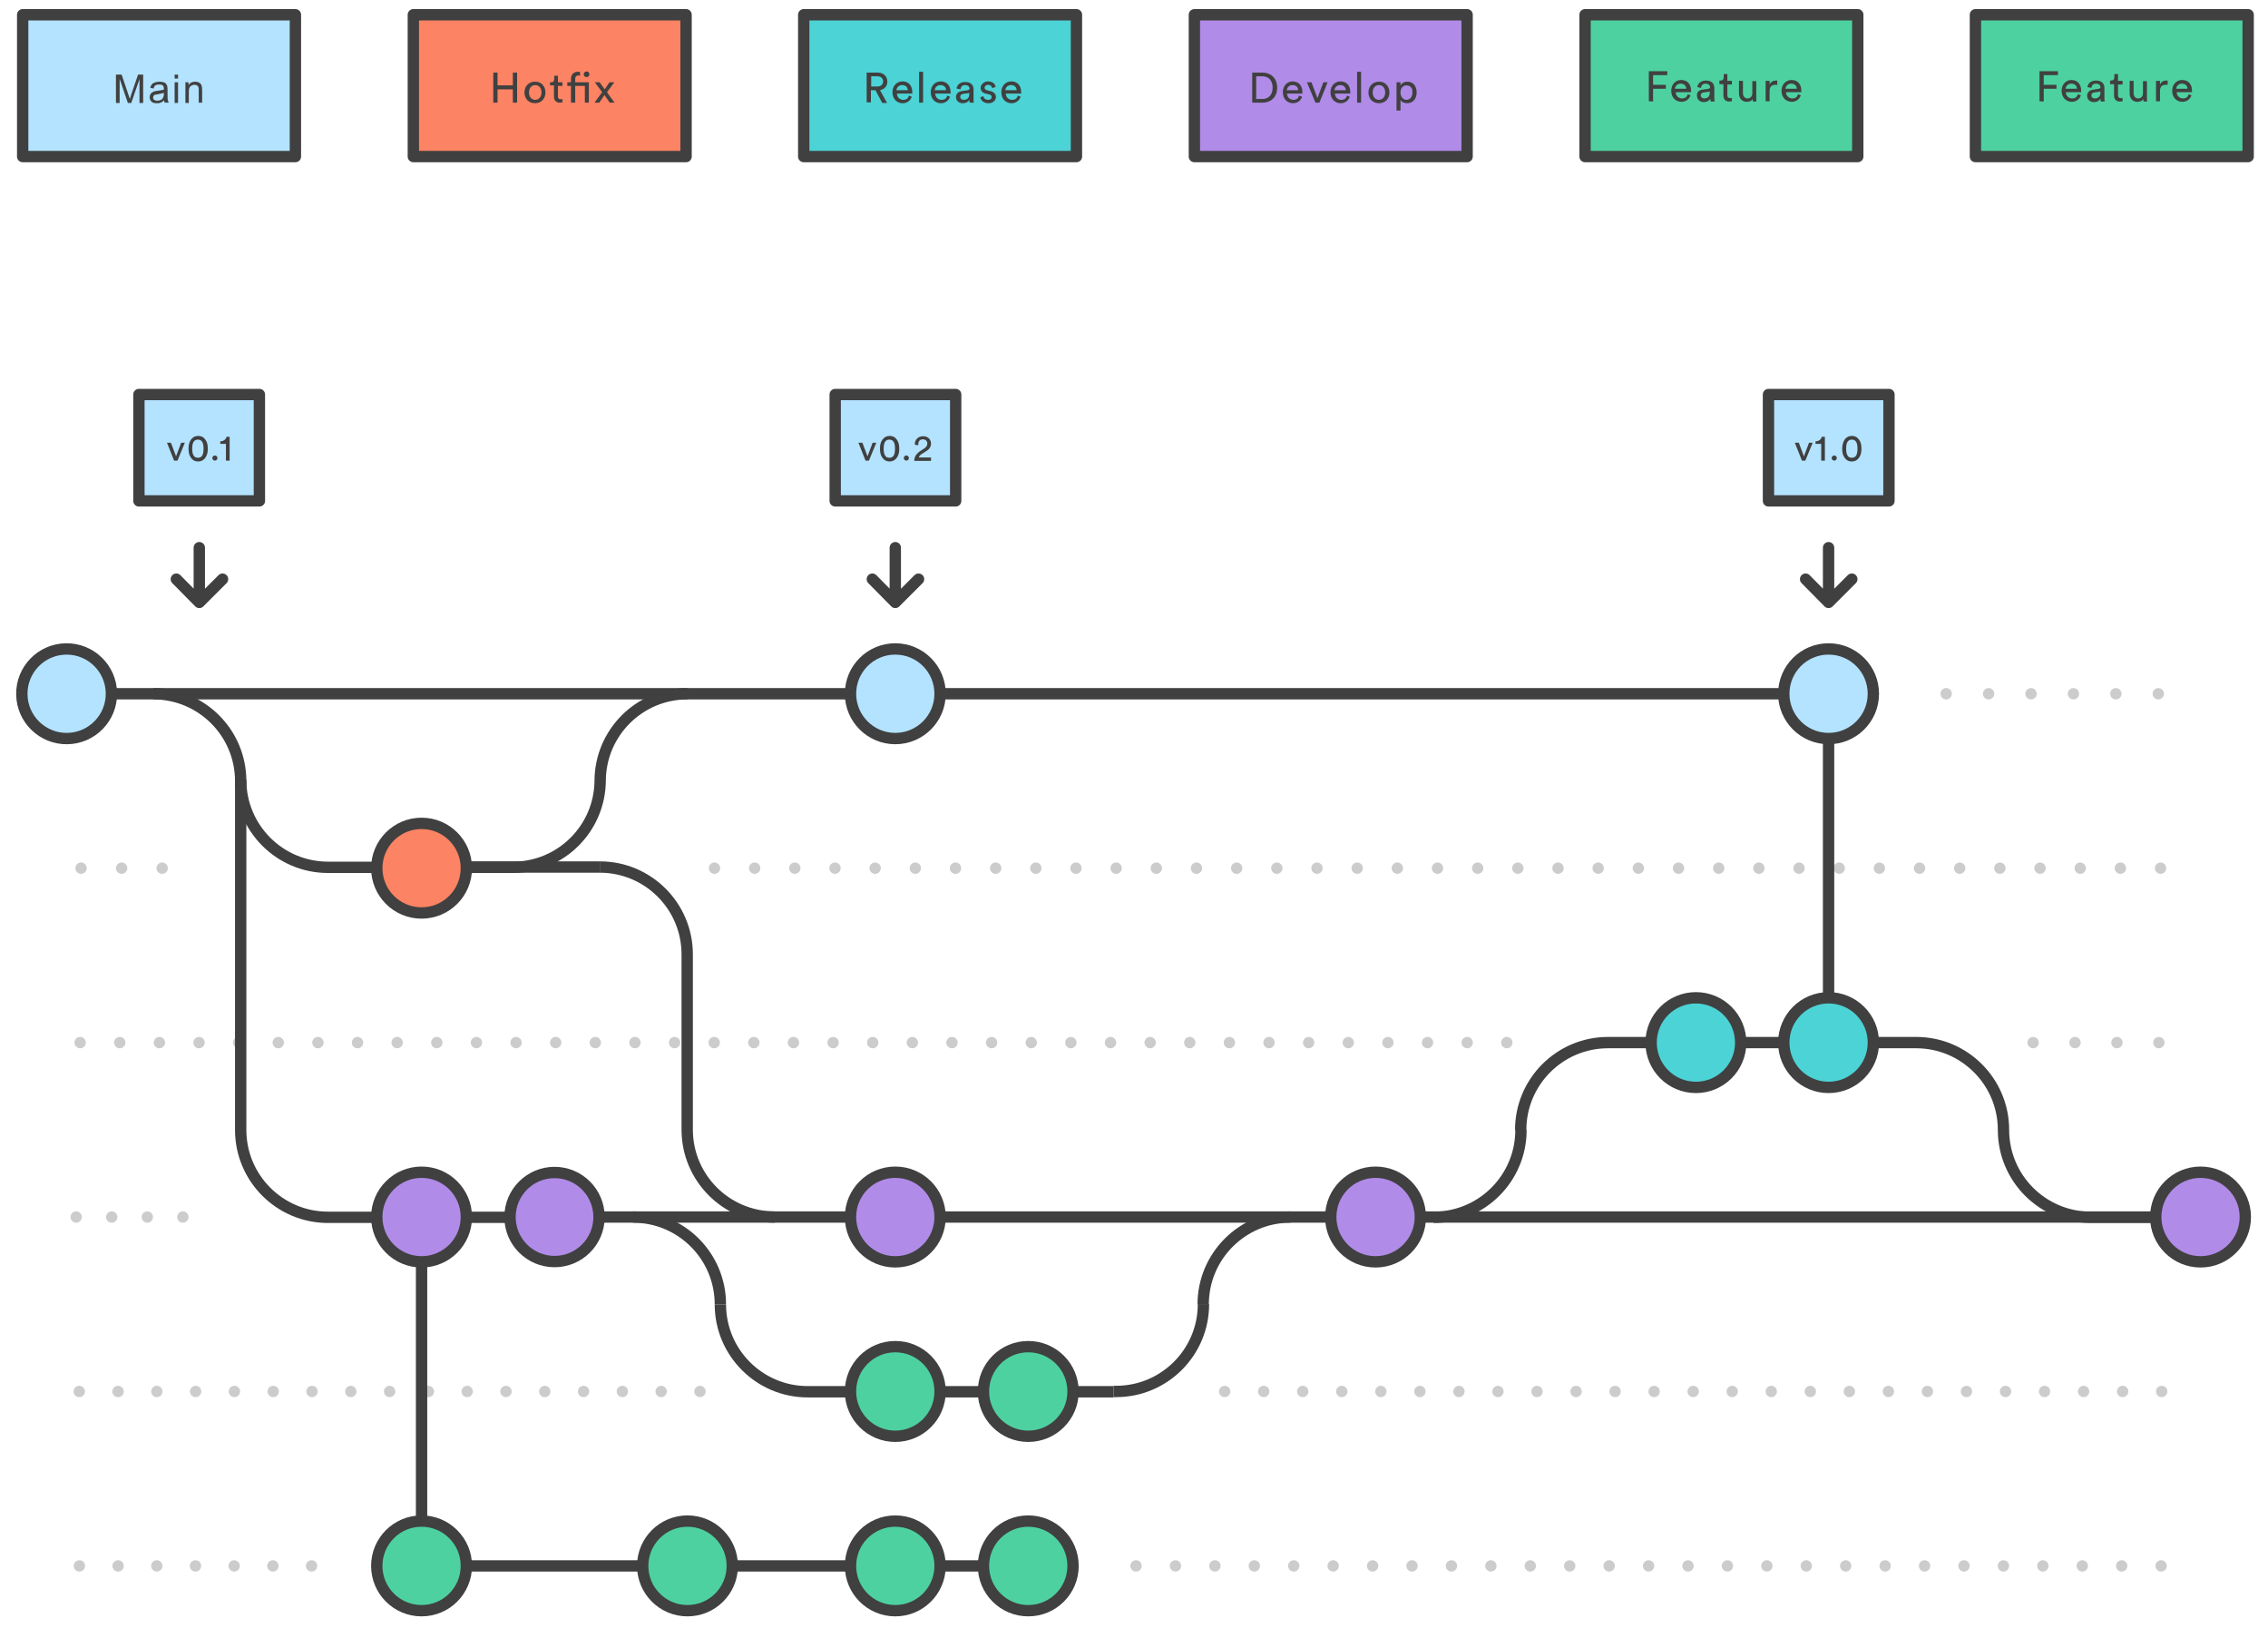
\includegraphics[width=0.7\textwidth]{capitolo3/gitflow.png}
  \caption{Rappresentazione grafica del workflow GitFlow}
  \textbf{Fonte}: \href{https://www.atlassian.com/git/tutorials/comparing-workflows/gitflow-workflow}{https://www.atlassian.com/git/tutorials/comparing-workflows/gitflow-workflow}
\end{figure}

È stato utilizzato questo \textit{workflow} misto per sfruttare al meglio le potenzialità che hanno le \textit{pull request} offerte dalla piattaforma GitHub, e la sistematicità che caratterizza GitFlow. Infatti, in GitFlow le fasi di sviluppo sono ben definite ed organizzate, associate ognuna ad un \textit{branch}. Questo permette una gestione migliore di tutto il processo di sviluppo, sia che si lavori in un \textit{team} composto da molte persone, sia che si lavori da solo.

\paragraph{GitHub}
GitHub è un servizio di \textit{hosting} per progetti \textit{software}, incentrato sull'utilizzo di Git. Permette anche l'integrazione in ogni \textit{repository} Git, di: \textit{Issue Tracking System}, strumenti per realizzare la \textit{Continuous Integration} e \textit{artifact repository}. 

Uno strumento molto potente ed innovativo che ha introdotto GitHub è la \textit{pull request}, ovvero una richiesta di aggiunta di modifiche che sono state apportate o da un collaboratore interno alla repository, richiedendo la fusione di un \textit{branch} con un altro attraverso questo strumento, oppure da un collaboratore esterno, il quale ha apportato le modifiche in un \textit{fork} del progetto. In seguito la \textit{pull request} dovrà essere approvata da uno dei proprietari della \textit{repository}. 

La \textit{pull request} effettuata da un collaboratore interno è importante anche per effettuare l'analisi statica del codice non automatica, dove una persona manualmente analizza il codice che deve essere approvato.

\paragraph{Issue Tracking System}
Il ITS (\textit{Issue Tracking System}) è uno strumento che facilita la gestione del processo di sviluppo e di \textit{change management}, attraverso la gestione di attività diverse (\textit{work item}). Ogni singola attività del progetto è gestita con un \textit{workflow} e mantenuta in un'unica \textit{repository}. Il ITS serve a condividere le informazioni con il \textit{team} di sviluppo, il \textit{project manager} e i vari \textit{stakeholders}. \\

Come ITS è stato scelto quello offerto da GitHub, il quale permette la definizione di \textit{Work Item}, anche chiamati \textit{issue}. Le \textit{issue} hanno le seguenti proprietà:
\begin{itemize}
  \item un codice univoco;
  \item lo stato, ovvero se è aperta o chiusa;
  \item un nome;
  \item una descrizione;
  \item chi la deve svolgere;
  \item la \textit{board} a cui è associata;
  \item la \textit{milestone} di cui fa parte.
\end{itemize}

Le funzionalità non terminano qui, infatti, come anche accennato precedentemente, il ITS permette la definizione di \textit{milestone} e la creazione di \textit{board}.

\paragraph{Continuous Integration}
La CI (\textit{Continuous Integration}) è una pratica che consiste nell'allineamento frequente degli ambienti di lavoro degli sviluppatori verso l'ambiente condiviso, dove ci sarà sempre il codice più aggiornato e funzionante. Per poter sfruttare questa pratica, è molto importante aver predisposto un ambiente che automatizzi l'esecuzione di test automatici per facilitare l'attività di verifica. \\

Durante il mio stage è stato utilizzato \textit{GitHub Action} come servizio per la programmazione di azioni che si verificano ad uno specifico evento e per automatizzare vari processi di lavoro. Tutte le \textit{action} sono definibili attraverso file di configurazione scritti nel linguaggio YAML.

\paragraph{Artifact repository}
Il \textit{artifact repository} è uno strumento per ottimizzare e storicizzare i \textit{file} utilizzati e prodotti durante lo sviluppo. In poche parole, si centralizza la gestione di tutti i \textit{file} binari, anche detti artefatti, generati e utilizzati durante la fase di \textit{build}. \\

\noindent Gli \textit{artifact repository} che sono stati utilizzati durante lo sviluppo sono:
\begin{itemize}
  \item \textbf{\textit{NPM}}: acronimo di \textit{Node Package Manager}, ha il compito di storicizzare tutti gli artefatti generati da applicativi basati sul \textit{framework} Node.js. Gli artefatti sono scaricabili e gestibili dall'omonimo strumento;
  \item \textbf{\textit{Maven Central Repository}}: \textit{artifact repository} ufficiale, dove vengono pubblicati tutti gli artefatti prodotti in seguito al processo di \textit{build} dello strumento Maven;
  \item \textbf{\textit{GitHub Artifact Repository}}: \textit{artifact repository} interna a GitHub, utilizzata per la pubblicazione degli artefatti prodotti in seguito al processo di \textit{build} dello strumento Maven. Nel \textit{GitHub Artifact Repository} sono stati caricati tutti gli \textit{smart contract} per Hotmoka e la libreria per l'integrazione con il \textit{back-end} NFTLab, in modo tale da facilitarne l'importazione e la gestione. Non è stata utilizzata la \textit{Maven Central Repository}, visto che questi artefatti sono interni al progetto e non hanno l'obiettivo di funzionare al di fuori del contesto NFTLab.
\end{itemize}

\subsubsection{Documento tecnico}
Per quanto riguarda la scrittura del documento tecnico e la realizzazione dei vari diagrammi UML, ho utilizzato, rispettivamente, il linguaggio Markdown e Mermaid. 

\textbf{Markdown} è un linguaggio di \textit{markup} con una sintassi del testo semplice progettata in modo che possa essere convertita in HTML. È perfettamente integrabile con la piattaforma GitHub, la quale mette a disposizione la lettura online di documenti scritti in Markdown.

\textbf{Mermaid}, invece, è uno strumento che permette di generare le immagini dei diagrammi UML a partire da un \textit{file} con estensione mmd. L'utilizzo di Mermaid ha facilitato di molto la realizzazione dei diagrammi richiesti, senza doversi occupare della parte grafica. In seguito le immagini generate sono state importate dentro il documento scritto in Markdown.

% \clearpage
\begin{figure}[h!]
  \centering
  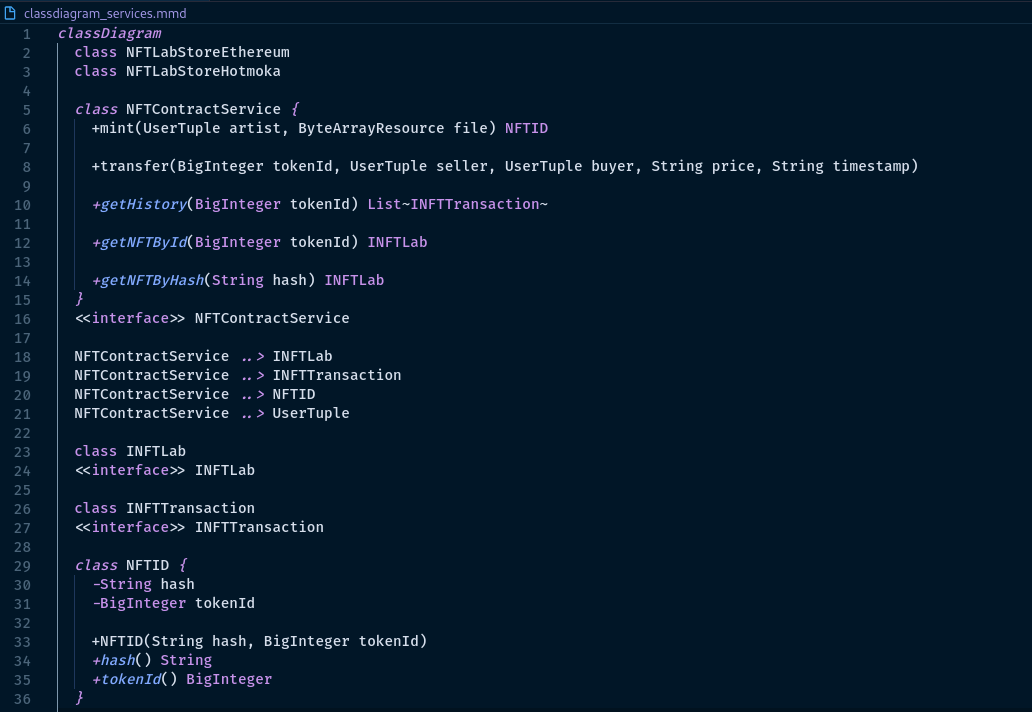
\includegraphics[width=\textwidth]{capitolo3/mermaid-example.png}
  \caption{Esempio di diagramma delle classi sviluppato con Mermaid}
  \textbf{Fonte}: \href{https://github.com/NFT-Lab/smart-contract-integration/blob/main/docs/classdiagram\_services.mmd}{https://github.com/NFT-Lab/smart-contract-integration/blob/main/docs/classdiagram\_services.mmd}
\end{figure}

\subsubsection{Ambienti di sviluppo}
Come ambienti di sviluppo sono stati utilizzati IntelliJ Idea per la scrittura di codice che riguardava il linguaggio Java e Visual Studio Code per quella che riguardava il linguaggio di programmazione Solidity.

\textbf{IntelliJ IDEA} è un ambiente di sviluppo integrato per il linguaggio di programmazione Java. Ha molte funzionalità che facilitano la gestione del codice, infatti esegue automaticamente il \textit{code refactoring} in base alle modifiche che si vogliono apportare, si integra perfettamente con lo strumento di versionamento GIT e gli strumenti di \textit{build automation} Maven e Gradle.

\textbf{Visual Studio Code}, invece, è un \textit{code editor} sviluppato su Electron, un \textit{framework} attraverso il quale è possibile sviluppare applicazioni \textit{desktop} utilizzando le tecnologie web. Appena installato non ha molte funzionalità, ma grazie alle numerose estensioni che sono state create e si possono installare, può essere considerato un IDE. Principalmente è stato utilizzato per lo sviluppo in Solidity, con estensioni che avviano lo strumento di analisi statica e formattazione del codice ad ogni salvataggio.

\subsubsection{Tecnologie usate}
Le tecnologie utilizzate durante il processo di sviluppo, tra cui linguaggi di programmazione, \textit{framework}, librerie, strumenti di \textit{build automation} e strumenti per l'analisi statica del codice, sono riportate di seguito.

\paragraph{HardHat}
HardHat è un ambiente di sviluppo per \textit{smart contract} in Solidity per Ethereum. Ha vari strumenti che facilitano di molto lo sviluppo ed i più importanti sono i seguenti:
\begin{itemize}
  \item possibilità di utilizzo di una \textit{blockchain} Ethereum temporanea e relativi \textit{wallet}, la quale annulla il \textit{block time} togliendo qualsiasi forma di \textit{proof of X}, durante la fase di testing, in modo da velocizzarla;
  \item possibilità di scrivere vari script in Typescript per eseguire il \textit{deploy} dello \textit{smart contract}, oppure semplicemente per comunicare con uno precedentemente caricato su varie reti Ethereum, come quella pubblica o una qualsiasi \textit{testnet};
  \item possibilità di scrivere tutti i \textit{test} utilizzando Typescript;
  \item integrazione con lo strumento solcover.js per ottenere il report del code coverage raggiunto.
\end{itemize}

\paragraph{Ganache}
Ganache è uno strumento per creare una \textit{blockchain} Ethereum locale non temporanea, con la quale interagire per svolgere vari \textit{test}. Anch'essa, come quella di Hardhat, annulla il \textit{block time} togliendo qualsiasi forma di \textit{proof of X} per velocizzare il \textit{testing}. Offre molte funzionalità, ma quella più importante è la possibilità di avere a disposizione moltissimi \textit{wallet} già forniti di Ether, con i quale comunicare con la \textit{blockchain}.

\clearpage
\begin{figure}[h!]
  \centering
  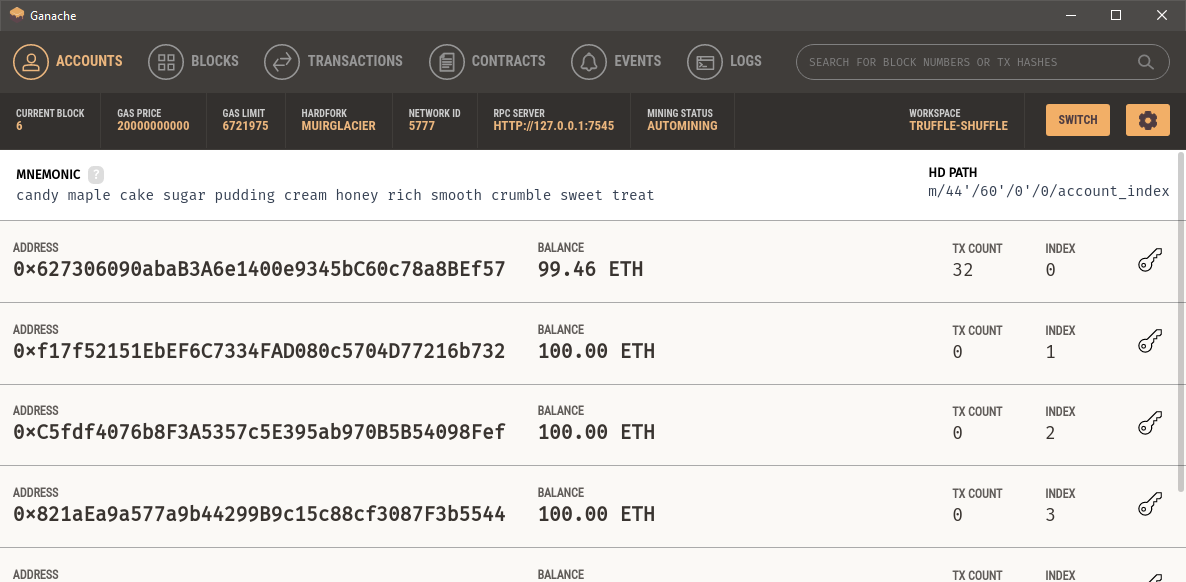
\includegraphics[width=\linewidth]{capitolo3/ganache.png}
  \caption{Schermata principale dello strumento Ganache}
\end{figure}

\paragraph{Web3J} 
Web3J è una libreria utilizzata da applicativi Java per comunicare con \textit{smart contract} per Ethereum.
Oltre ad essere una libreria, offre anche uno strumento che genera automaticamente a partire da un contratto scritto in Solidity, una classe Java dove sono stati implementati tutti i metodi per la comunicazione con quello specifico \textit{smart contract}, offrendo anche la possibilità di eseguire il \textit{deploy} o il caricamento di un contratto precedentemente inserito. 

\paragraph{Maven}
Maven è uno strumento di \textit{build automation} e gestione di progetti \textit{software} basati su Java. Effettua automaticamente il \textit{download} delle librerie Java e \textit{plug-in} Maven, dai vari \textit{repository} definiti,scaricandoli in locale. Questo permette di recuperare in modo uniforme i vari \textit{file} \textit{JAR} e di poter spostare il progetto da un ambiente all'altro, avendo la sicurezza di utilizzare sempre le stesse versioni delle librerie. Utilizza un \textit{file} XML chiamato POM (\textit{Project Object Model}), dove vengono descritte le dipendenze tra il progetto e le varie versioni delle librerie necessaire, nonché le dipendenze fra di esse. È stato utilizzato per la gestione di tutti i progetti Java sviluppati durante il percorso di stage, ovvero la libreria per l'integrazione e gli \textit{smart contract} per Hotmoka.

\paragraph{JUnit5}

JUnit5 è la versione 5 del \textit{framework} più famoso per la scrittura di \textit{test} nel linguaggio di programmazione Java. È stata utilizzata per la scrittura di test d'unità, d'integrazione e di sistema. Utilizzato insieme al plugin per Maven chiamato JaCoCo, permette di creare il report del \textit{code coverage} raggiunto e pubblicarlo su vari servizi come \textit{Coveralls}.

\paragraph{Mockito}
Mockito è la libreria più popolare per la realizzazione di oggetti \textit{mock} nel linguaggio di programmazione Java. Nella programmazione orientata agli oggetti, l'isolamento dei test unitari viene ottenuto utilizzando oggetti che simulano il comportamento degli oggetti reali. Questi oggetti vengono chiamati, come detto in precedenza, \textit{mock}.

\paragraph{Mocha}
Mocha è un \textit{framework} per la scrittura di test in JavaScript, eseguito su Node.js. I test Mocha vengono eseguiti in serie, per produrre report flessibili e accurati. Inoltre le eccezioni non rilevate vengono mappate ai casi di test corretti. Per facilitare il \textit{testing}, è stato associato alla libreria di asserzioni \textbf{Chai}, la quale ha il compito di verificare che il risultato ottenuto corrisponda a quello atteso. Chai presenta molte funzioni e metodi per confrontare l'output di un determinato test con il suo valore atteso.

\paragraph{Solhint}
Solhint è uno strumento per l'analisi statica di codice Solidity. È stato utilizzato durante la fase di sviluppo dello \textit{smart contract} in Solidity con le regole che vengono raccomandate dallo strumento stesso. In più è stato associato ad uno strumento di \textit{code formatting}, chiamato \textbf{prettier}, per definire le regole di formattazione del progetto.


\paragraph{Checkstyle}
Checkstyle è uno strumento che permette di eseguire l'analisi statica di codice Java. Si integra perfettamente con Maven e verrà eseguito automaticamente durante la fase di verifica, prima di quella di compilazione. Ho utilizzato le regole definite da Google, le quali sono impostate come predefinite.
Inoltre Checkstyle permette di generare un \textit{report} dello stato dell'analisi statica del codice, in modo tale da poterlo utilizzare con strumenti come SonarQube che hanno il compito di elaborare questo tipo di \textit{report}.
